\documentclass[a4paper,11pt]{article}

\usepackage[english]{babel} 
\usepackage[utf8]{inputenc}
\usepackage[cyr]{aeguill}
\usepackage{stmaryrd}

\usepackage{lmodern} %Type1-font for non-english texts and characters
\usepackage{caption}
\usepackage{subcaption}

\usepackage{graphicx}
\usepackage{hyperref}
\usepackage{listings}

\usepackage{epstopdf}

%% Math Packages 
\usepackage{amsmath}
\usepackage{amsthm}
\usepackage{amsfonts}
\usepackage{amssymb}
\usepackage{mathrsfs}
\usepackage{pst-all}
\usepackage{lscape}
\usepackage{pdfpages}
\usepackage{mathabx}


\usepackage{color, colortbl}
\definecolor{lightgray}{gray}{0.85}
\usepackage{multirow}
\usepackage[Algorithme]{algorithm}
\usepackage[noend]{algpseudocode}
\usepackage{tikz}

%\renewcommand{\algorithmicdo}{\textbf{faire}}
%\renewcommand{\algorithmicwhile}{\textbf{tant que}}


\usepackage{a4wide} %%Smaller margins = more text per page.
\usepackage{fancyhdr} %%Fancy headings

\setcounter{secnumdepth}{5}
\setcounter{tocdepth}{5}


\DeclareMathOperator*{\argmax}{arg\,max}
\DeclareMathOperator*{\argmin}{arg\,min}
\graphicspath{{/Users/melisandezonta/Documents/Documents/Documents/GTL_courses_second_semester/Computer-Vision/PS3-all/PS3-input/}}




\usepackage{listings}
\usepackage{color}
 
\definecolor{codegreen}{rgb}{0,0.6,0}
\definecolor{codegray}{rgb}{0.5,0.5,0.5}
\definecolor{codepurple}{rgb}{0.58,0,0.82}
\definecolor{backcolour}{rgb}{0.95,0.95,0.92}
 
\lstdefinestyle{mystyle}{
    backgroundcolor=\color{backcolour},   
    commentstyle=\color{codegreen},
    keywordstyle=\color{magenta},
    numberstyle=\tiny\color{codegray},
    stringstyle=\color{codepurple},
    basicstyle=\footnotesize,
    breakatwhitespace=false,         
    breaklines=true,                 
    captionpos=b,                    
    keepspaces=true,                 
    numbers=left,                    
    numbersep=5pt,                  
    showspaces=false,                
    showstringspaces=false,
    showtabs=false,                  
    tabsize=2
}
 
\lstset{style=mystyle}

\begin{document}

%\pagestyle{fancy}

\begin{titlepage}
\vspace*{\stretch{1}}

\begin{center}

\includegraphics[scale=0.4]{GT_logo.jpeg}
\end{center}
\vspace*{\stretch{1}}
\hrulefill
\begin{center}\bfseries\huge
   Computer Vision \\
   CS 6476 , Spring 2018\\
   \end{center}
  \begin{center}\bfseries\large
     PS 3\\
    \hrulefill
\end{center}
%\hfill
\vspace*{1cm}
\begin{minipage}[t]{0.6\textwidth}
  \begin{flushleft} \large
    \emph{Professor : }\\
    Cedric Pradalier \\
  \end{flushleft}
\end{minipage}
\begin{minipage}[t]{0.3\textwidth}
  \begin{flushright} \large
    \emph{Author :} \\
    Melisande Zonta \\
  \end{flushright}
\end{minipage}
\vspace*{\stretch{2}}
\begin{flushright}
       \today 
\end{flushright} 
\end{titlepage}

\tableofcontents
\clearpage

\section{Calibration}

The first part of this problem set consists in determining the projection matrix of a camera based on the location of known 3D points in the world and their corresponding 2D points in the image.

\subsection{Projection Matrix Computation}


The computation of the projection matrix is done using the svd (singular value decomposition) trick, as visible in the code below.

Indeed as the problem is presented as the product of the matrix M and the homogenous vector of 3D points : 

$$
\begin{bmatrix}
u_{i}  \\
v_{i}   \\
1  \\
\end{bmatrix} 
=
\begin{bmatrix}
m_{00} & m_{01}  & m_{02} & m_{03} \\
m_{10} & m_{11}  &  m_{12} & m_{13}  \\
m_{20} & m_{21}  & m_{22}  & m_{23} \\
\end{bmatrix}
\begin{bmatrix}
X_{i} \\
Y_{i}  \\
Z_{i}  \\
1
\end{bmatrix}
$$

The above equality provides one pair of equations for each point such that :

$$
\left[
\begin{array}{cccccccccccc}
X_1 & Y_1& Z_1 & 1 &   0    & 0     & 0     & 0 & -u_{1}X_{1} & -u_{1}Y_{1} & -u_{1}Z_{1} & -u_{1} \\
0    & 0      & 0     & 0  & X_1 & Y_1& Z_1 & 1 & -v_{1}X_{1} & -v_{1}Y_{1} & -v_{1}Z_{1} & -v_{1} \\
\vdots & \vdots & \vdots & \vdots & \vdots & \vdots   & \vdots & \vdots & \vdots & \vdots & \vdots & \vdots \\
X_n & Y_n& Z_n & 1 & 0 & 0 & 0 & 0 & -u_{n}X_{n} & -u_{n}Y_{n} & -u_{n}Z_{n} & -u_{n} \\
0      & 0 & 0 & 0 & X_1 & Y_1& Z_1 & 1 & -v_{1}X_{1} & -v_{1}Y_{1} & -v_{1}Z_{1} & -v_{1} \\
\end{array}
\right]
\begin{bmatrix}
m_{00} \\ m_{01}  \\ m_{02} \\ m_{03} \\
m_{10} \\ m_{11}  \\  m_{12} \\ m_{13}  \\
m_{20} \\ m_{21}  \\ m_{22}  \\ m_{23} 
\end{bmatrix}
=
\begin{bmatrix}
0  \\
0
\end{bmatrix}
$$

This is a homogenous set of equations under the form $Ax = 0$. We can apply the singular value decomposition to A and then reshapedinto a 3 x 4 matrix that corresponds to our projection matrix.

\lstset{style=mystyle}
\lstinputlisting[language=Python, firstline=39, lastline=64]{/Users/melisandezonta/Documents/Documents/Documents/GTL_courses_second_semester/Computer-Vision/PS3-all/PS3-code/Functions.py}
\lstinputlisting[language=Python, firstline=29, lastline=36]{/Users/melisandezonta/Documents/Documents/Documents/GTL_courses_second_semester/Computer-Vision/PS3-all/PS3-code/Functions.py}

Applying this function to the sets of normalized 2D and 3D points, we get the following matrix:
$$
\begin{matrix}
[ [ &0.45827553 & -0.29474238  & -0.01395749  & 0.00402579& ]\\
 [ &-0.05085589 & -0.0545847 &  -0.5410599  & -0.05237592&]\\
 [ &0.10900958 & 0.1783455  & -0.04426782  & 0.5968205&]] \\
\end{matrix}
$$
Finally, projecting the last 3D point given in the file (pts3d-norm.txt), we get the following projection on the 2D image:
$$
\begin{matrix}
[ &0.14190586 & -0.45183985  & 1.  & ]\\
\end{matrix}
$$
These coordinates match the ones given in the file (pts2d-norm-pic-a.txt) with a residual (distance) of 0.0016.


\subsection{Random Sets}

We now compute the projection matrix for random sets of point pairs with different sizes (8, 12 and 16).

We repeat the computation 10 times for each size of set.

For each iteration, we take 4 more random pairs of points (outside the ones used for computing M) and compute the average residual.

We also output the projection matrix corresponding to the lowest residual for each size of set.

The following code is used:

\lstset{style=mystyle}
\lstinputlisting[language=Python, firstline=18, lastline=65]{/Users/melisandezonta/Documents/Documents/Documents/GTL_courses_second_semester/Computer-Vision/PS3-all/PS3-code/ps3-1-2.py}

%Add the result for normalized points
We get the results presented on figure \ref{ps3-1-2}.
 \begin{figure}[h!]
\begin{center}
	\includegraphics[height= 1\textwidth]{ps3-1-2-result}
\end{center}
\caption{ Results of the random sets. }
\label{ps3-1-2}
\end{figure}

We notice that for a larger set of points, the average residuals decreases. 
This means that our projection matrix tends to give more accurate projections when 4 more pairs of points are used in the least squares solving.

This is true in this case because there is no outliers in the input data, i.e. the pairs of points are accurately matched. Should the input data be more realistic (noise and outliers), the number of pairs used for the computation should be
chosen more carefully.

Indeed, a larger number of matching points will reduce the impact of the Gaussian noise, but if outliers are present, the resulting estimation of M will be impacted no matter the number of pairs used.

\subsection{Camera Center Computation}

The next step is to compute the location of the camera center in the 3D world, based on the previously determined projection matrix.

The coordinates are computed using the following function:

\lstset{style=mystyle}
\lstinputlisting[language=Python, firstline=66, lastline=66]{/Users/melisandezonta/Documents/Documents/Documents/GTL_courses_second_semester/Computer-Vision/PS3-all/PS3-code/Functions.py}

The resulting estimate shown below effectively matches the coordinates given in the problem set description.

$$
\begin{matrix}
[ &-1.51576097 & -2.35511764  & 0.28244984  & ]\\
\end{matrix}
$$

When applying the M matrix found in the previous function with the set of points pts2d-pic-b.txt and  pts3d.txt, we obtain the following location of the camera in the 3D world : 
$$
\begin{matrix}
[ &303.11692085 & 307.20745856  & 30.42544351  & ]\\
\end{matrix}
$$


\section{Fundamental Matrix Estimation}


The objective of the second part of this problem set is to determine the fundamental matrix based on locations of pairs of matching points in two images.

\subsection{Full Rank Fundamental Matrix Estimation}

As a first step, we solve for the full rank fundamental matrix (Ft) using the singular value decomposition method as previously, that is visible in the code below.
The resulting matrix is reshaped in a 3 x 3 form.

\lstset{style=mystyle}
\lstinputlisting[language=Python, firstline=68, lastline=82]{/Users/melisandezonta/Documents/Documents/Documents/GTL_courses_second_semester/Computer-Vision/PS3-all/PS3-code/Functions.py}

Applying this function to the points in our files (pts2d-pic-a.txt and pts2d-pic-b.txt) we get the following result:

%fix the problem of those exponentielle
$$
\begin{matrix}
[ [ &-6.60698417e-07 & 7.91031621e-06  & -1.88600198e-03 & ]\\
 [ & 8.82396296e-06 & 1.21382933e-06 &  1.72332901e-02  &]\\
 [ & -9.07382302e-04 & -2.64234650e-02  & 9.99500092e-01 &]] \\
\end{matrix}
$$

\subsection{Fundamental Matrix Computation}


In order to get the actual fundamental matrix from this full rank estimate, we compute the Singular Value Decomposition (SVD) of Ft.
$$U\Sigma V^{T} = F_{t}$$


To estimate the rank 2 matrix, we first set the smallest singular value (the last one in our case, since numpy.linalg.svd sorts them in a decreasing order). Then we compute the fundamental matrix F using the following product:

$$F = U\Sigma ' V^{T}$$

The following code implements this computation:

\lstset{style=mystyle}
\lstinputlisting[language=Python, firstline=17, lastline=20]{/Users/melisandezonta/Documents/Documents/Documents/GTL_courses_second_semester/Computer-Vision/PS3-all/PS3-code/ps3-2-2.py}

As a result, and based on the previously determined $F_{t}$ matrix, we get the following fundamental matrix F:

%fix the problem of those exponentielle
$$
\begin{matrix}
[ [ &-5.35883058e-07 & 7.89972529e-06  & -1.88480998e-03 & ]\\
 [ & 8.83820595e-0 & 1.21802118e-06 &  1.72276843e-02 &]\\
 [ &-9.08539026e-04 & -2.64201801e-02  & 1.00000000e+00 &]] \\
\end{matrix}
$$

\subsection{Epipolar Lines Estimation and Drawing}

Now we want to draw the epipolar lines on both input images.

We use the homogeneous coordinates duality between points and lines to get to the desired result.

We first need to compute the coordinates of the left and right edges of the image. This is achieved by computing the cross product of respectively the top and bottom left corner coordinates and top and bottom right corner coordinates, as follows (where m and n are the width and height of the image):

$$ L_{l} = 
\begin{bmatrix}
0 \\ 0 \\ 1
\end{bmatrix} 
\times
\begin{bmatrix}
 0 \\ n \\ 1
\end{bmatrix}
$$

$$ L_{r} = 
\begin{bmatrix}
 m \\ 0 \\ 1
\end{bmatrix} 
\times 
\begin{bmatrix}
 m \\ n \\ 1
\end{bmatrix}
$$

Next, for each 2D point, we compute the epipolar line using the dot product of
F (respectively $F^T$ ) and the point homogeneous coordinates.

$$ L_{i} = 
F
.
\begin{bmatrix}
 x_{j} \\ y_{j} \\ 1
\end{bmatrix}
$$

$$ L_{j} = 
F^{T}
.
\begin{bmatrix}
 x_{i} \\ y_{i} \\ 1
\end{bmatrix}
$$

Then we compute the homogeneous coordinates of the intersection points of $L_{i}$
with $L_l$ and $L_r$  using a cross product:

$$P_{il} = L_{i} \times L_{l}$$
$$P_{ir} = L_{i} \times L_{r}$$
We finally draw the line on the image based on the cartesian coordinates of those
two points.

The previous equations were implemented in this code : 

\lstset{style=mystyle}
\lstinputlisting[language=Python, firstline=85, lastline=110]{/Users/melisandezonta/Documents/Documents/Documents/GTL_courses_second_semester/Computer-Vision/PS3-all/PS3-code/Functions.py}

Computing the epipolar lines for the image A (using the image B 2D points coordinates) results in Figure \ref{ps3-2-3}a.
Similarly, computing for the image B (using the image A 2D points coordinates) gives us the Figure \ref{ps3-2-3}b .

 \begin{figure}[H]
\begin{center}
\begin{tabular}{c}
	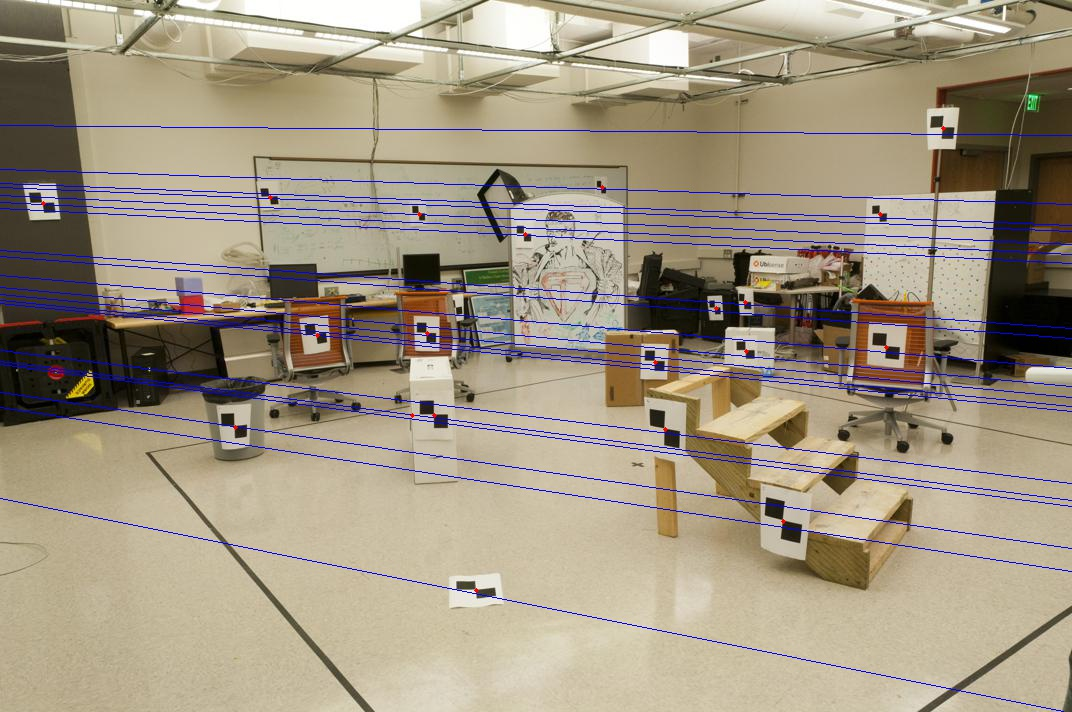
\includegraphics[width=1\textwidth]{ps3-2-3-a.jpg}\\
	a\\
	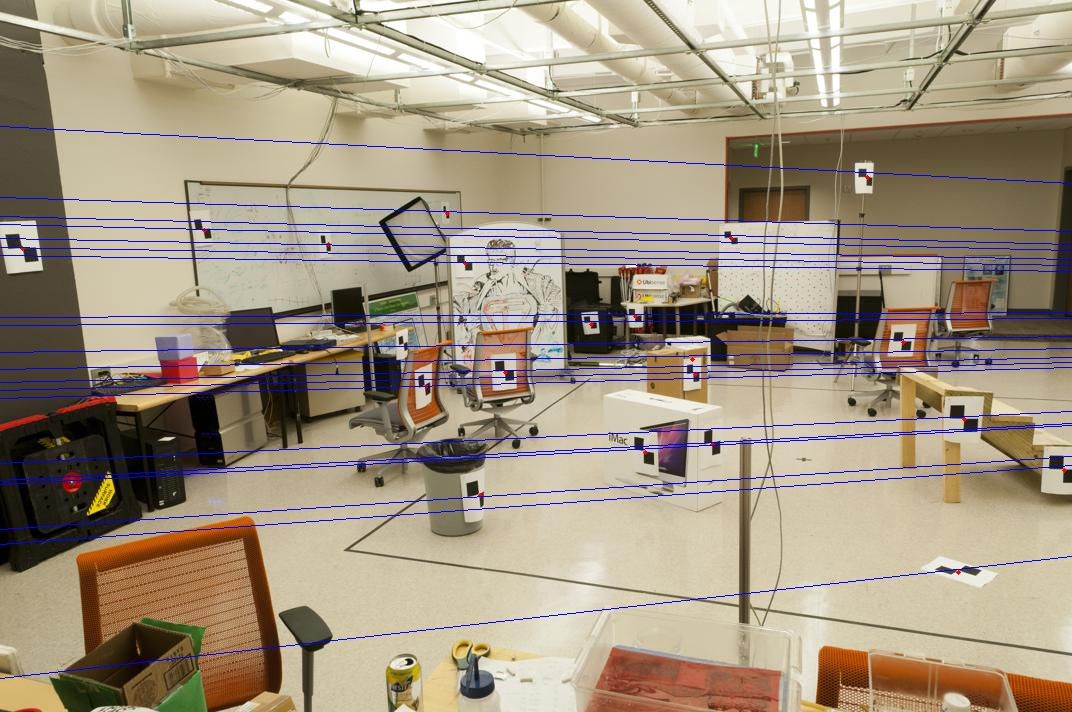
\includegraphics[width=1\textwidth]{ps3-2-3-b.jpg}\\
	b
\end{tabular}
\end{center}
\caption{ 
\textit{a}. ps3-2-3-a.  \textit{b}. ps3-2-3-b. }
\label{ps3-2-3}
\end{figure}

\subsection{2D Points Normalization}


In order to correct the innacuracies of our initial estimate, we need to normalize the 2D points using a scale and offset transformation.

We first compute the transformation matrix using the inverse of the maximum coordinate value as a scale and the opposite of the means as offset, as shown in the code below:

\lstset{style=mystyle}
\lstinputlisting[language=Python, firstline=118, lastline=129]{/Users/melisandezonta/Documents/Documents/Documents/GTL_courses_second_semester/Computer-Vision/PS3-all/PS3-code/Functions.py}

The two transformation matrices we obtain for the A and B 2D points are the following:

The transformation matrix for the 2D points of image A is : 
$$
\begin{matrix}
[ [ & 1.06044539e-03& 0.00000000e+00. & -5.80063627e-01 & ]\\
 [ & 0.00000000e+00 & 1.06044539e-03 &  -1.30434783e-01 &]\\
 [ &0.00000000e+00 & 0.00000000e+00 & 1.00000000e+00 &]] \\
\end{matrix}
$$


The transformation matrix for the 2D points of image B is
$$
\begin{matrix}
[ [ &9.39849624e-04 &0.00000000e+00  & -4.55357143e-01& ]\\
 [ & 0.00000000e+00 & 9.39849624e-04 &  -1.26879699e-01 &]\\
 [ &0.00000000e+00 & 0.00000000e+00  & 1.00000000e+00 &]] \\
\end{matrix}
$$


Then we compute an intermediate fundamental matrix (Fh) using the normalized 2D points as an input:

$$
\begin{matrix}
[ [ &-0.01998282 &0.28265631  & -0.0759324& ]\\
 [ &0.18524791 & -0.05514497 &  0.5972918 &]\\
 [ &-0.00377719 & -0.72075553  &0.01782818 &]] \\
\end{matrix}
$$

\subsection{Accurate Fundamental Matrix Computation}

The last step is to compute the more accurate fundamental matrix F based on the previously determined Fh.

$$F = T_{b}^T.F_{h}.T_{a}$$

We get the following fundamental matrix:

$$
\begin{matrix}
[ [ &-1.99160637e-08  &2.81712007e-07  & -9.51215321e-05& ]\\
 [ &1.84629034e-07 & -5.49607394e-08 &  4.67132566e-04 &]\\
 [ &-1.92810921e-05  & -8.93391641e-04  & 9.70542710e-02&]] \\
\end{matrix}
$$

Finally, we can draw again the epipolar lines on both images using the new fundamental matrix.
The result, more accurate, is visible in Figure \ref{ps3-2-5}a. and Figure b.
Obviously it didn't work, and I couldn't figure why since it seemed I wrote every formula correctly.

 \begin{figure}[H]
\begin{center}
\begin{tabular}{c}
	\includegraphics[width=1\textwidth]{ps3-2-5-a.jpg}\\
	a\\
	\includegraphics[width=1\textwidth]{ps3-2-5-b.jpg}\\
	b
\end{tabular}
\end{center}
\caption{ 
\textit{a}. ps3-2-5-a.  \textit{b}. ps3-2-5-b. }
\label{ps3-2-5}
\end{figure}

\end{document}